\documentclass[../main.tex]{subfiles}
\graphicspath{{\subfix{../../images/}}}

\begin{document}

USB is a protocol and interface by which data is transmitted between computers and computer peripherals. it can be seen in many places, like between your computer and a mouse, a cable to connect your phone to the computer, USB microphones, audio devices, hubs, and other possible peripherals.

\subsection{USB-A}

Usually referred to as just USB or USB Type-A apart from the name USB-A, the cross-section of the connector typically looks like a black rectangle with an empty section with a silver coating around it, with 2 holes. Inside the cable, there exists 4 wires:

\begin{figure}[h]
    \centering
    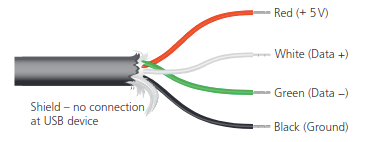
\includegraphics[width=0.6\textwidth]{usb_inside}
    \caption{The inside of a USB cable, taken from the textbook}
    \label{fig:usb_inside}
\end{figure}

Figure \ref{fig:usb_inside} shows the 4 wires in a USB-A cable:

\begin{itemize}
    \item A wire carrying \textbf{+5 volts}, usually in red,
    \item \textbf{Ground}, or the negative terminal usually in black
    \item \textbf{Green and white}, for serial communication (data- and data+).
\end{itemize}

And the corresponding port and connector looks like so:

\begin{figure}[h]
    \centering
    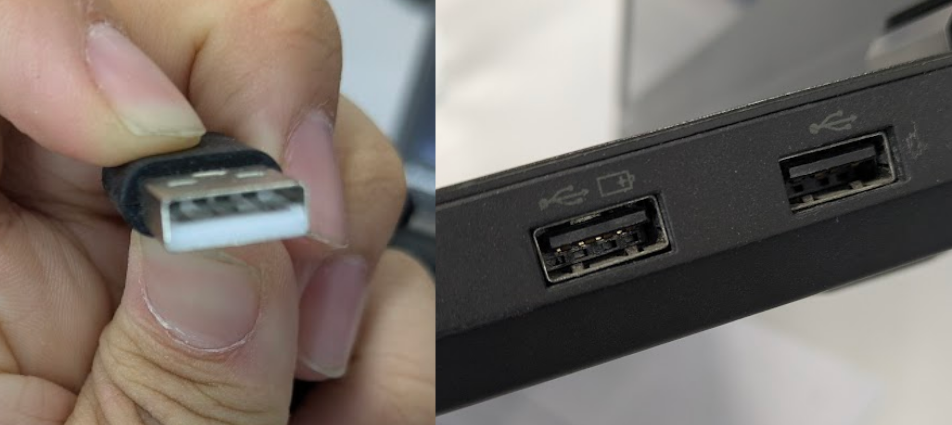
\includegraphics[width=0.6\textwidth]{usb_port_and_connector}
    \caption{The connector and port of USB-A}
    \label{fig:usba_port_and_connector}
\end{figure}

Since this connector is by far the most common connector used in computers, you may very likely have one on your device. Simply check the sides and or back
for an example\footnote{Unfortunately, if you possess a newer Apple computer, Apple took away the USB-A ports to make you purchase adapters. Look for another device or an adapter for an example in that case}.

\subsection{Benefits and Drawbacks of USB-C}

Note that one only needs to know a few advantages and disadvantages; some are quite specific.

\textbf{Benefits include}:
\begin{itemize}
    \item USB-A is very common; seen on most computers and devices
    \item The connector itself is more durable due to its thickness
    \item Since the connector only fits in one way, incorrect connections cannot be made
    \item The USB protocol makes use of error correction\footnote{As it should be.}\footnote{If any errors are found, the data is to be re-transmitted.}
    \item If one needs more ports, they can choose to connect a \emph{USB Hub} which splits one USB port into many, similar to an Ethernet switch)
\end{itemize}

\textbf{Drawbacks include}:
\begin{itemize}
    \item Standard USB-A only supports cables up to 5 meters, requiring extensions for cables to go further.
    \item The connector is one way, making it difficult to insert without looking at the port.
    \item Very early USB standards, like USB1 may not be supported by the latest computers.
    \item By far the most common USB-A standard, USB2, found in the vast majority of devices from 2000 till now, only supports 480Mbits/s, meaning that ethernet adapters and other applications that may require higher speed data transfer cannot be done.
\end{itemize}

\subsection{USB-C}

USB-C, USB Type-C, or just Type-C is the most common USB connector on newer computing devices; all Apple devices after \textasciitilde 2016 have USB-C, and computers between around \textasciitilde 2016 til \textasciitilde 2020 have \emph{only} USB-C ports.

This connection is called USB, however the connector looks quite different from standard USB-A:

\begin{figure}[h]
    \centering
    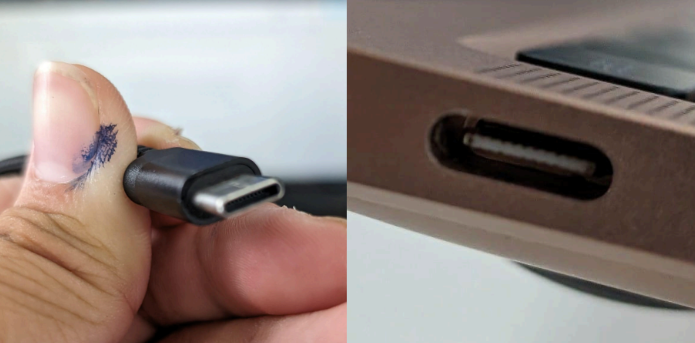
\includegraphics[width=0.6\textwidth]{usbc_port_and_connector.png}
    \caption{The connector and port of USB-C}
    \label{fig:usbc_port_and_connector}
\end{figure}

As seen in Figure \ref{fig:usbc_port_and_connector}, USB-C takes on more of a rounded shape, smaller than USB-A and is a \emph{Symmetrical Connector}, meaning it can be inserted both ways.

\newpage

\paragraph{Quirks}

\begin{itemize}
    \item USB-C can carry \emph{A video signal}\footnote{Through the DisplayPort standard.}, meaning external monitors and TVs can be connected.
    \item USB-C supports a standard called USB-C PD (Power Delivery). The textbook\footnote{Since USB-C standards change relatively rapidly,
          the textbook version should be beter for the exams as that is in the syllabus} states USB-C can deliver a 20 volt 5 amp
          (therefore 100W) power signal to change devices at a high wattage.
    \item USB-C supports extremely high data transfer rates. The textbook states that it can deliver up to 40 gigabits to second, however the latest standard\footnote{USB4 Gen 2} supports up to 120 gigabits per second asymmetrically and 80Gbit/s symmetrically.
    \item USB-C is fully backwards compatible\footnote{This generally means that a newer thing fully supports all the features of the older thing} with USB-A, one just needs a simple adapter with the correct lanes connected to make use of this feature.
    \item the USB-C connector is also used by Thunderbolt, which is a way to connect PCIe Express devices through USB\footnote{This is very niche and may not come up in tests, but it is good to know}. Professional audio devices or graphics cards can be connected through this port.
\end{itemize}

\subsection{Benefits and Drawbacks of USB-C}

Note that one only needs to know a few advantages and disadvantages; some are quite specific.

\textbf{Benefits include}:
\begin{itemize}
    \item USB-C can carry more types of signals, such as a video signal, power delivery, and Thunderbolt.
    \item USB-C can deliver much faster speeds for high volume data transfers, like between film cameras and computers.
    \item It can be inserted into a port both ways; it makes connecting devices in less accessible locations more convenient.
    \item It supports far more ports and devices, like DisplayPort, through adapters.
\end{itemize}

\textbf{Drawbacks include}:
\begin{itemize}
    \item It is relatively rare on older devices; only around 2016-2018 did computer manufacturers put USB-C ports on their devices. A lot of them, even to this day do not support data transfer through the port; only power delivery.
    \item Since USB-C has so many standards (Video, USB, PCI through Thunderbolt, different levels of Power Delivery and even no-data cables), it is confusing as some ports are incapable of delivering thunderbolt, while others are incapable of delivering video, etc.
    \item USB-A has colors (White/Black and Blue for USB2 and 3 respectively) to determine the generation; and for USB type B the connectors are physically different to determine the generation. USB-C does not have any way of differentiating, so one must memorize the capabilities of their USB-C device to know the supported generation.
\end{itemize}

\end{document}
